%% Capitol 4
% \part{FreeRTOS}
% \label{part:freertos}
\chapter{Conceptes bàsics de FreeRTOS}
\label{ch:FreeRTOS}
% \chapter{Sistemes Operatius de Temps Real}

En el Firmware per sistemes encastats que hem vist fins ara es basen en un bucle infinit on es van executant les tasques a fer. Això acostuma a ser prou bo per sistemes senzills, com ara llegir d'un \gls{ADC} i decidir alguna cosa, o actuar sobre una sortida segons el valor d'un sensor, etc.

Per sistemes més complexos o amb requeriments crítics, s'acostuma a fer servir un Sistema Operatiu per gestionar diferents tasques.
\begin{remark}

Un sistema és de Temps Real quan el temps de resposta del sistema a un event extern està fitada. És a dir, es pot saber i està garantit el temps total entre que
succeeix un esdeveniment i el sistema genera una sortida.

Un exemple típic és el d'un airbag. El temps màxim, sigui el que sigui que el sistema estigui fent entre que es detecta l'accident i es dispara l'airbag està garantit i limitat.

Un Sistema Operatiu de Temps Real (RTOS en anglès) és un Sistema Operatiu que està dissenyat per garantir aquesta fita de temps.
\end{remark}
\glsreset{RTOS}
En aquest llibre farem servir \gls{FreeRTOS} \cite{freertos}, un \gls{RTOS} de codi obert àmpliament utilitzat. En el cas de EFM32 i STM32 els fabricants ens proporcionen el {\em porting} de FreeRTOS a les seves plataformes.

\begin{remark}
 Se'n diu {\em porting} al fet d'adaptar un codi a una plataforma específica. Per exemple, en el cas del FreeRTOS, cal adaptar una sèrie de funcions per a que tot el sistema funcioni, com ara la gestió dels rellotges, la gestió de tasques, etc.
\end{remark}


En tot \gls{OS} (i \gls{RTOS}) les feines a fer per part del sistema es reparteixen en diferents tasques (\glspl{task} en anglès). Aquestes tasques s'executen “simultàniament” i, per tant, cal repensar bé tot el sistema abans de començar a escriure el codi.

En sistemes encastats, un SO (o RTOS) no ofereix totes les funcionalitats a les que estem acostumats quan sentim parlar d'un SO. Així, normalment el que ens ofereix un RTOS és:

\begin{itemize}
 \item Gestió de tasques: Creació, execució, estat de les tasques, prioritats de tasques, etc.
 \item Comunicació entre tasques: Semàfors, cues, etc.
 \item Gestió de temps: Timers, {\em timeouts}, {\em delays}, etc.
\end{itemize}

Les tasques són les unitats bàsiques de funcionament i és on s'implementen les funcionalitats del sistema.

\section{Tasques}

Una tasca és el que es coneix com a procés en els Sistemes Operatius de propòsit general. Per tant, una tasca serà l'estructura mínima de codi en que es divideix una aplicació. Aquestes tasques seran les que el planificador o {\em scheduler} del Sistema Operatiu anirà executant i retirant d'execució segons certes condicions que veurem a continuació.

Bàsicament una tasca pot estar en l'estat {\em Running} (executant-se), {\em Ready} (disponible per ser executada) o {\em Blocked} (no preparada perquè està esperant a algun esdeveniment)\footnote{També hi ha l'estat {\em Suspended} on la pròpia tasca demana sortir de la llista de {\em Ready}}. A la Figura~\ref{fig:taskstate} es pot veure quins estats pot tenir una tasca en FreeRTOS \cite[92]{FreeRTOSBook}.


\begin{figure}
 \centering
 \fbox{\color{ocre}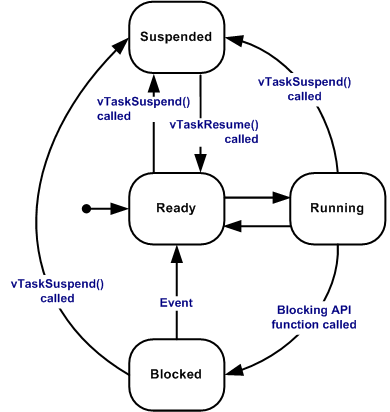
\includegraphics[width=0.85\textwidth, keepaspectratio]{imatges/tskstate.png}}
 \caption{Estats possibles d'una tasca. \copyright\ FreeRTOS}
 \label{fig:taskstate}
\end{figure}

Les tasques són funcions amb un bucle infinit i una inicialització prèvia i en cap cas la funció pot retornar. Si una tasca ja no és necessària, es pot eliminar per part el RTOS, però no pot acabar retornant la funció per si mateixa.
Pel cas de \gls{FreeRTOS}, tenen l'aspecte que es mostra al Llistat~\ref{task}.

\index{OneTask()}
\begin{lstlisting}[caption={Esquelet d'una tasca},style=customc,label=task]
static void OneTask(void *pParameter) {
  (void) pParameter;
  /* Init */

  while(1) {
    /* bucle infinit */
  }
}
\end{lstlisting}

Una aplicació basada en un RTOS és un conjunt de tasques funcionant concurrentment i comunicades entre elles. El \gls{RTOS} ens dona diferents funcions que ens permeten: comunicar tasques entre elles o bloquejar-se per un cert temps.

\subsection{Prioritats}

Quan es creen les tasques, a cada una se li assigna una certa prioritat. Aquesta prioritat marcarà quina de les tasques de l'estat {\em Ready} passarà a executar-se {\em Running} a cada moment. A \gls{FreeRTOS} les tasques amb una prioritat d'un valor més baix tenen menor prioritat (0 és el valor més baix i menys prioritari). Diferents tasques poden tenir la mateixa prioritat.

Existeix una tasca {\em Idle} que s'executa cada cop que cap altra tasca està a l'estat {\em Ready}. Aquesta tasca té la prioritat més baixa, de valor 0 i per tant només s'executa quan cap tasca està llesta. La tasca {\em Idle} sempre està disponible per executar-se a qualsevol moment.

Per saber més sobre prioritats i com assignar-les a les tasques, veieu \fullref{sec:priorities_RMA}.
\subsection{L'ús de l'{\em stack} en un S.O.}
\label{sub:StackOS}
Per crear una tasca, un dels paràmetres que es passa a la funció {\bf xTaskCreate}\index{xTaskCreate()} és la mida de l'\gls{stack} per la tasca que s'està creant.

Se'n diu {\em stack} a la regió de memòria assignada a una tasca que s'utilitza bàsicament per dues coses:
\begin{itemize}
 \item guardar els valors dels paràmetres de les diferents crides a funcions que faci la tasca
 \item emmagatzemar el seu context quan el SO retira la tasca d'execució.
\end{itemize}

Aquest \gls{stack} normalment es gestiona com una pila (amb els mètodes {\em push} i {\em pop}) i acostuma a situar-se al final de la memòria i “créixer cap avall”.

A priori, és molt difícil saber quant {\em stack} farà servir una tasca, així que el més habitual és donar un valor per defecte prou gran i després, durant el funcionament normal, observar quanta se'n fa servir realment.

Per saber el nivell màxim a on s'ha arribat a l'{\em stack} de cada tasca, FreeRTOS fa servir un mètode una pel peculiar: a l'inicialitzar la tasca (i el seu {\em stack}) omple l'{\em stack} amb un valor predeterminat i conegut. Després, quan ja està funcionant el nostre sistema, només cal comptar quantes posicions de l'{\em stack} mantenen el valor conegut. Si s'acosta a 0 voldrà dir que la tasca està fent servir la majoria de l'espai de l'{\em stack}.

Per activar aquesta funcionalitat cal editar el fitxer {\bf FreeRTOSConfig.h} i definir la macro {\bf configCHECK\_FOR\_STACK\_OVERFLOW} amb el valor 2 i la macro {\bf uxTaskGetStackHighWaterMark} a 1.

Activant la primera de les macros, el sistema operatiu també controla que no s'intenti accedir fora de l'{\em stack}. D'aquesta manera podem saber si cal més {\em stack}, però no si ens en sobra ni quanta. En activar aquesta opció cal definir una funció de hook que s'anomeni {\bf vApplicationStackOverflowHook()}\index{vApplicationStackOverflowHook()} i que es cridarà cada cop que es detecti un error en accedir l'{\em stack}.

%\section{Scheduler}

% {\bf taskYIELD()}\index{taskYIELD()}


\section{El temps en un RTOS}
\label{sec:RTOS_time}
Habitualment un RTOS ha de portar un control del temps per decidir quina tasca s'ha d'executar, saber quan desbloquejar una tasca, etc.

Normalment es basen en el concepte de \gls{tick}. Un {\em tick} es genera de forma periòdica (normalment fent servir algun Timer) i la freqüència d'aquest {\em tick} ens marca el temps mínim que pot manegar el RTOS.

En el cas de FreeRTOS, a cada {\em tick} es deixa d'executar la tasca que està {\em running} i s'executa el planificador del RTOS. Si aquest planificador detecta que una tasca més prioritària està a punt per ser executada (estat {\em ready}), la posarà a executar ({\em running}) enlloc de la que hi havia fins feia un moment.

La freqüència d'aquest {\em tick} pot variar molt segons el sistema que tinguem, però acostuma a anar entre els 1000 Hz i els 50Hz. Segons la freqüència del {\em tick} tindrem un sistema més ràpid de resposta en segons quins casos a canvi d'alentir lleugerament l'execució general del sistema i de tenir menys resolució en les funcions de control de temps.

\subsection{Funcions per controlar el temps}

Tot OS proporciona una sèrie de funcions per gestionar el temps, això és:
\begin{itemize}
 \item bloquejar una tasca durant un cert temps determinat.
 \item controlar el {\em timetout} a certes crides del mateix.
\end{itemize}

\subsubsection{\em Delays}
Les funcions {\bf vTaskDelay()}\index{vTaskDelay()} i {\bf vTaskDelayUntil()}\index{vTaskDelayUntil()} són les dues funcions que ens permeten bloquejar la tasca que la crida durant el temps que s'especifica com a paràmetre.

Aquestes dues funcions faran que la tasca entri immediatament a l'estat {\em blocked} i restarà en aquest estat durant tota l'estona que s'especifiqui. Un cop hagi passat aquest temps la tasca passarà a l'estat {\em Ready}.

El paràmetre que rep la funció {\bf vTaskDelay()}\index{vTaskDelay()} és el nombre de {\em ticks} que es vol que la tasca estigui {\em blocked}. Com més precís sigui el {\em tick} del sistema (més freqüència) més acurat podrà ser aquest {\em delay}.

Cal veure que segons la prioritat de la tasca en qüestió i de la prioritat de la tasca que s'estigui executant, aquesta tasca pot romandre en l'estat {\em Ready} un temps indefinit.

\subsubsection{\em Timeout}
A les funcions d'accedir a un recurs compartit, com un semàfor o una cua, apareix un paràmetre que és el temps (en {\em Ticks}) que la tasca que accedix esperà a poder realitzar l'operació. Així, si s'especifica un temps de 100 mil·lisegons per llegir d'una cua, la funció retornarà passat aquest temps si la cua està buida i ningú hi ha escrit res o retornarà tant bon punt algú hi escrigui alguna dada.

\section{Interrupcions en FreeRTOS}
\label{ch:FreeRTOSIRQ}

FreeRTOS deixa el maneig de les interrupcions a mans del desenvolupador, demanant unes certes condicions.

Cal tenir en compte que les interrupcions són esdeveniments totalment asíncrons i imprevisibles i que prenen el control de forma automàtica. Això fa que mentre està funcionant una \gls{ISR} el {\em kernel} del Sistema Operatiu no es pot executar i que, quan acabi d'executar la ISR, si no fem res, tornarà el control cap a la tasca que s'estava executant. Això pot provocar que una ISR alliberi un recurs o posi disponible una dada i que una tasca d'alta prioritat passi a l'estat {\em Ready} però el {\em kernel}, com que no s'executa, no pugui passar-li l'execució i se segueixi amb la taca menys prioritària que s'estava executant.

Per això les funcions per accedir a recursos com semàfors o cues des d'una \gls{ISR} tenen un paràmetre extra, que informa si s'ha despertat una tasca més prioritària. Si és el cas, cal que el codi de la ISR faci un {\bf portYIELD\_FROM\_ISR()}\index{portYIELD{\_}FROM{\_}ISR()} per cridar al {\em kernel} del Sistema Operatiu (veure Llistat~\ref{ISRYield}).

\index{any{\_}IRQHandler()}\index{xSemaphoreGiveFromISR()}\index{portYIELD{\_}FROM{\_}ISR()}
\begin{lstlisting}[style=customc,caption=Codi ISR d'exemple,label=ISRYield]
void any_IRQHandler(void) {
  BaseType_t xHigherPriorityTaskWoken = pdFALSE;

  ...
  /* Toggle semaphore */
  xSemaphoreGiveFromISR(semaphore_button_0, &xHigherPriorityTaskWoken);

  portYIELD_FROM_ISR(xHigherPriorityTaskWoken);
}
\end{lstlisting}

Aquesta funció de {\em yield} retorna de la ISR i executa el {\em kernel} si la variable passada té un valor diferent a {\bf pdFALSE}.


Sempre es diu que les \glspl{ISR} han de ser el més curtes possibles, això és pels següents motius:
\begin{itemize}
 \item Mentre s'està executant una \gls{ISR} no es pot executar cap tasca, per molt prioritària que sigui.
 \item Depenent de l'arquitectura, mentre s'està executant una ISR la resta d'\glspl{IRQ} estan desactivades.
 \item Algunes arquitectures poden permetre anidar interrupcions, cosa que augmenta la complexitat i la incertesa de tot el sistema. Quan més curta sigui la ISR més improbable que això passi.
\end{itemize}

És per això que les bones pràctiques diuen que el codi dins una \gls{ISR} hi hagi poc codi i es facin servir semàfors o cues per notificar tasques on s'executin les operacions pertinents amb les prioritats adequades.

\chapter{Primer exemple amb FreeRTOS}
\label{sec:FreeRTOS_exemple_1}
El \href{https://github.com/mariusmm/cursembedded/tree/master/Simplicity/FreeRTOS_Blink}{primer exemple} és el nostre vell conegut ‘Hello World' per embedded, és a dir, blinkar un LED.

L'exemple consisteix en una sola tasca que s'encarrega de blinkar el LED. Com totes les tasques, consisteix en un bucle infinit on s'inclou tota la funcionalitat de la tasca (Llistat \ref{HelloWorldFreeRTOSTask}).

\index{TaskLedToggle()}\index{LedToggle()}\index{vTaskDelay()}
\begin{lstlisting}[caption={Tasca TaskLedToggle per FreeRTOS},style=customc,label=HelloWorldFreeRTOSTask]
static void TaskLedToggle(void *pParameter) {
  (void) pParameter;

  for (;;) {
    LedToggle();
    vTaskDelay(pdMS_TO_TICKS(500));
  }
}
\end{lstlisting}

Aquesta tasca fa servir una funció del RTOS ({\bf vTaskDelay()}\index{vTaskDelay()}) que bloqueja la tasca per un determinat temps. Així doncs, aquesta tasca tant sols farà Toggle al LED cada mig segon. Cal fixar-se que aquesta funció rep com a paràmetre el nombre de {\em ticks} a esperar-se. Aquest número es calcula amb la macro {\bf pdMS\_TO\_TICKS()}\index{pdMS\_TO\_TICKS()}, que passa de mil·lisegons a {\em ticks}.

Al {\bf main()}\index{main()} el que veiem és que, després de la inicialització habitual hem de crear les tasques que tingui el nostre sistema i tot seguit engegar el FreeRTOS (Llistat \ref{HelloWorldFreeRTOSMain}).

\index{main()}\index{xTaskCreate()}\index{vTaskStartScheduler()}
\begin{lstlisting}[caption={Main HelloWorld per FreeRTOS},style=customc,label=HelloWorldFreeRTOSMain]
main() {
  ...
  /* Create our first task */
  xTaskCreate(TaskLedToggle, (const char *) "LedToggle",
        configMINIMAL_STACK_SIZE, NULL, TOGGLE_TASK_PRIORITY, NULL);

  /* Start FreeRTOS Scheduler */
  vTaskStartScheduler();
  ...
}
\end{lstlisting}

La funció {\bf xTaskCreate()\index{xTaskCreate()}} rep diferents paràmetres:
\begin{enumerate}
 \item Punter a la funció que implementa la tasca
 \item Nom que li posem a la tasca (per debug)
 \item \gls{stack} reservat per la tasca (veure~\fullref{sub:StackOS})
 \item Punter a paràmetres per la tasca
 \item Prioritat de la tasca
 \item {\em Handle} a la tasca creada
\end{enumerate}

Aquesta funció retorna {\bf pdPASS} si s'ha creat la tasca o un error en cas contrari.

La funció {\bf vTaskStartScheduler()\index{vTaskStartScheduler()}}, que en condicions normals no retorna mai, comença l'execució del FreeRTOS i aquest, al seu torn, executarà la nostra tasca.

% A continuació veurem diversos exemples de com comunicar tasques fent servir semàfors, mutex i cues.

% \chapter{Tasques a S.O.}




%%%%%%%% AMPLIAR

\chapter{Comunicació entre tasques}

En aquest capítol es detallen diferents mecanismes de sincronització i comunicació entre tasques en un Sistema Operatiu encastat.

Qualsevol RTOS que porti aquest nom ens oferirà una sèrie de mecanismes per a comunicar tasques entre elles. Els mecanismes més habituals són:
\begin{itemize}
 \item Semàfors: Una tasca no pot agafar un semàfor fins que una altre no l'allibera.
 \item Cues: Permeten enviar informació d'una tasca a una altra.
 \item {\em Mutex}: Permet protegir un recurs compartit de manera que només una tasca el faci servir en un moment donat.
\end{itemize}

N'hi ha d'altres, com esperar i enviar esdeveniments o grups d'esdeveniments, {\em mailboxes}, senyals, etc. que acostumen a ser pròpies de cada \gls{OS} concret.

\section{Semàfors}
Un semàfor és un dels mecanismes de comunicació entre tasques mes habituals dels que ofereix un OS. En essència el funcionament d'un semàfor és tal que una tasca prova d'agafar el semàfor i es quedarà esperant que una altra tasca doni el semàfor o ho tornarà a provar més endavant \cite[244]{EmbeddedDictionary} \cite[187]{programmingembedded}.

Habitualment es fan servir per sincronitzar almenys dues tasques que comparteixen el semàfor o per protegir una secció crítica.

\subsection{Semàfors a FreeRTOS}
A FreeRTOS tenim diferents tipus de semàfors:

\begin{itemize}
 \item {\em Binary}: pot tenir només l'estat ‘agafat' o ‘donat'. Es fan servir per sincronitzar tasques.
 \item {\em Counting}: s'emmagatzema un número, que s'incrementa en ‘donar' el semàfor i es redueix en ‘agafar' el semàfor. Sempre que tingui un valor positiu es podrà ‘agafar' el semàfor. Serveix per portar un compte del nombre de recursos disponibles.
 \item {\em Mutex}: són una variant dels semàfors binaris que inclouen mecanismes d'herència de prioritats. Es fan servir per implementar l'exclusió mútua. En parlarem més endavant, a \fullref{sec:Mutex}.
\end{itemize}

\subsection{Exemple amb semàfors}
\label{sub:semafors_exemple}
A \href{https://github.com/mariusmm/cursembedded/tree/master/Simplicity/FreeRTOS_Semaphore}{l'exemple} hi ha una tasca que es queda esperant a agafar un semàfor i quan l'aconsegueix fa un {\em toggle} del LED (Veure Llistat~\ref{semaphore_task_example}).

\index{TaskLedToggle()}\index{xSemaphoreTake()}\index{LedToggle()}
\begin{lstlisting}[style=customc,caption=Tasca amb semàfor d'exemple,label=semaphore_task_example]
static void TaskLedToggle(void *pParameter) {
  (void) pParameter;

  for (;;) {
    xSemaphoreTake(semaphore_button_0, portMAX_DELAY);
    LedToggle();
  }
}
\end{lstlisting}

La funció {\bf main()}\index{main()} crida la funció {\bf BSP\_Init()}\index{BSP{\_}Init()} que configura els GPIOs corresponents als botons i es registra una \gls{ISR} ({\bf GPIO\_EVEN\_IRQHandler()}\index{GPIO{\_}EVEN{\_}IRQHandler()}) pel botó 0, que ‘dóna' el semàfor en quan es prem el corresponent botó a la PCB (Llistat~\ref{ISR_semaphore}).

Després es crea el semàfor que compartiran la tasca i la ISR i tot seguit es crea la tasca com ja hem vist a l'exemple anterior..
Per últim s'engega el {\em kernel} del RTOS.

Cal notar que les funcions per agafar o donar un semàfor són diferents segons estiguem a una tasca o a una \gls{ISR}. En el cas de la ISR, la funció de donar al semàfor ens indica si hi ha alguna tasca que cal desbloquejar perquè l'està esperant. En cas que sigui cert, cal fer un {\em yield} des de la \gls{ISR} per a que el planificador ({\em scheduler}) del RTOS pugui actuar immediatament.

\index{xSemaphoreGiveFromISR()}\index{portYIELD{\_}FROM{\_}ISR()}
\begin{lstlisting}[caption=ISR del botó 0,style=customc,label=ISR_semaphore]
ISR() {
  ...
  /* Toggle semaphore */
  xSemaphoreGiveFromISR(semaphore_button_1, &xHigherPriorityTaskWoken);
  portYIELD_FROM_ISR(xHigherPriorityTaskWoken);
}
\end{lstlisting}

Tant en aquest exemple com en els següents el {\em timeout} de les crides és {\bf portMAX\_DELAY}. Aquesta macro serveix per indicar a la funció que es vol esperar un temps infinit a que l'operació es pugui realitzar. En aquest cas, la funció cridada no retornarà fins que pugui executar l'acció i bloquejant la tasca el temps necessari. D'aquesta mena de crides a funcions se'n diu crides bloquejants.

\begin{exercise}
Es pot provar d'implementar un codi que blinki el LED tantes vegades com vegades s'ha premut el botó 0. És pot fer amb un semàfor tipus {\em counting semaphore}.
\end{exercise}


\section{Cues}
\label{sec:queue}
Hem vist que els semàfors són útils per sincronitzar tasques i per protegir zones d'exclusió mútua, però no ens donen cap solució senzilla per enviar informació o dades d'una tasca a una altra. Aquesta comunicació és per les cues \cite[102]{FreeRTOSBook}.

Ens podem imaginar una cua com un recurs compartit entre dues o més tasques, on unes poden escriure-hi i d'altres hi poden llegir dades. Habitualment (en FreeRTOS és així), les cues s'implementen amb una estructura tipus FIFO (First-In First-Out) protegida de tal manera que no hi hagi cap \gls{race condition} durant el seu funcionament\footnote{S'anomena {\em race condition} al malfuncionament d'un codi donat que està executant-se en un entorn multitasca. Aquesta mena d'errors poden ser molt difícils de detectar i arreglar}.

A més, per tal de poder implementar sistemes d'una forma senzilla, els accessos a les cues poden ser bloquejants: la tasca que fa l'accés es quedarà bloquejada fins que pugui fer l'accés (esperar a poder escriure una dada, donat que no podia perquè la cua era plena) o esperar fins que hi hagi una dada (perquè s'ha intentat llegir de la cua quan aquesta era buida).

Les operacions habituals a una cua son:
\begin{itemize}
 \item Crear una cua ({\em create}): normalment cal especificar quin tipus de dades ha d'emmagatzemar la cua i quants espais o llocs cal preparar.
 \item Inserir una dada ({\em send}): afegir (si hi ha lloc) una dada nova a la cua.
 \item Llegir dada ({\em receive}): treure una dada (si n'hi ha) de la cua.
\end{itemize}

Altres operacions poden ser:
\begin{itemize}
 \item Mirar si hi ha una dada disponible (sense llegir-la) ({\em peek}).
 \item Esborrar tot el contingut de la cua ({\em reset}).
 \item Inserir una dada al principi de la cua (sense complir que la cua és una FIFO).
\end{itemize}

Les cues són recursos que poden ser compartits per vàries tasques, podent-hi escriure diferents tasques o \glspl{ISR} i poder llegir-la també diferents tasques, tot i que això de tenir múltiples tasques llegint d'una cua no és gaire habitual.

Per saber quina mida han de tenir les cues, veieu \fullref{sec:mida_cues}.
\subsection{Exemple amb cues}
\label{sub:cues_exemple}
A \href{https://github.com/mariusmm/cursembedded/tree/master/Simplicity/FreeRTOS_Queue}{l'exemple de cues} hi ha una sola tasca que fa {\em blinkar} el \gls{LED} segons una variable. Aquesta variable s'obté de llegir (o intentar-ho) una cua. Aquesta cua (anomenada {\em queue\_buttons}) l'escriuen les dues \gls{ISR} associades als dos botons. Una envia el valor corresponent a 250 ms i l'altre ISR envia el valor que correspont a 1000 ms (Llistat~\ref{Queue_example_ISR}).

\index{xQueueSendFromISR()}\index{portYIELD{\_}FROM{\_}ISR()}
\begin{lstlisting}[style=customc, label=Queue_example_ISR, caption=Part del codi d'una de les ISRs]
...
/* Send the data to the Queue */
xQueueSendFromISR(queue_buttons, (void* ) &new_delay,
		&xHigherPriorityTaskWoken);

/* Awake a task ? */
portYIELD_FROM_ISR(xHigherPriorityTaskWoken);
...
\end{lstlisting}


En aquest cas, la tasca fa servir la funció {\bf xQueueReceive()}\index{xQueueReceive()} amb un valor de 0 a l'últim paràmetre, que és el temps en {\em ticks} que ha d'esperar-se a rebre un valor en el cas que la cua estigui buida (veure Llistat~\ref{queue_example_main}).

\index{xQueueReceive()}\index{vTaskDelay()}\index{LedToggle()}\index{TaskLedToggle()}
\begin{lstlisting}[style=customc,label=queue_example_main, caption=Part principal de la tasca TaskLedToggle]
for (;;) {
  /* try to get new delay time from queue */
  if (xQueueReceive(queue_buttons, &recv_delay, (TickType_t ) 0)) {
    my_delay = recv_delay;
  }

  /* wait for m_delay & toggle the LED */
  vTaskDelay(my_delay);
  LedToggle();
}
\end{lstlisting}

En aquest exemple volem que encara que no hi hagi dada a la cua, la tasca segueixi executant-se. Per saber si la funció de rebre dades ha obtingut una dada nova, cal comprovar si ha retornat \gls{pdTRUE}. Si retorna \gls{pdFALSE} és que ha acabat el temps d'espera (en el nostre cas 0 {\em ticks}) i no ha pogut extreure un nou valor de la cua. Aquest és un exemple d'accés no bloquejant a una cua.

Les cues cal crear-les abans d'utilitzar-les cridant a la funció {\bf xQueueCreate()}\index{xQueueCreate()}. Aquesta funció crea la cua amb la longitud desitjada i amb la capacitat indicada (Llistat~\ref{queue_example_create}).
Usualment això es crea a la funció {\bf main()}\index{main()} o, en tot cas, abans d'engegar el Sistema Operatiu.

\index{xQueueCreate()}
\begin{lstlisting}[style=customc, label=queue_example_create, caption=Creació d'una cua]
/* Create Queue */
queue_buttons = xQueueCreate(QUEUE_LENGTH, sizeof(uint32_t));
\end{lstlisting}

% A les cues de FreeRTOS hi ha una particularitat que cal tenir en compte, i és que les funcions que accedeixen a la cua treballen amb punters a les dades, no amb les dades mateixes. Això es fa per evitar còpies de les dades innecessàries a l'stack (ho veurem més endavant).
%
% Per això a l'exemple tenim:
% \begin{lstlisting}[style=customc,label=ISR_semaphore]
%  xQueueSendFromISR(queue_buttons, (void* ) &new_delay,
%    &xHigherPriorityTaskWoken);
% \end{lstlisting}
%
% on new_delay està definit de tipus uint32_t.
%
% Això vol dir que la variable on es guarden les dades que s'envien per la cua cal que segueixi viva fins que la tasca que rep la dada pugui llegir-la. Així, cal vigilar amb variables automàtiques:

\section{Mutex}
\label{sec:Mutex}
Quan tenim un recurs, {\em driver}, memòria compartida, secció crítica o qualsevol altre recurs que només es pot fer servir per una sola tasca a cada moment, cal muntar un mecanisme d'exclusió mútua que ens asseguri que no tindrem cap problema \cite[244]{FreeRTOSBook}.

Aquest mecanisme és molt similar a un semàfor binari però cal incloure algun mecanisme per prevenir la inversió de prioritats. Aquest mecanisme és el Mutex (d'aquí els ve el nom: {\em Mutual Exclusion}). Els Mutex implementen un mecanisme d'herència de prioritats de tal manera que si una tasca d'alta prioritat està esperant un Mutex que té una tasca de baixa prioritat, aquesta última veu augmentada la seva prioritat a la mateixa prioritat que la tasca d'alta prioritat mentre té el Mutex per tal que tingui més oportunitat d'alliberar-lo ja que altres tasques amb prioritats entre mig poden bloquejar la tasca de baixa prioritat \footnote{Aquest problema és el conegut {\em inversió de prioritats} que pot donar molts mal de caps si no es detecta a temps}.

Per l'ús correcte d'un Mutex, el que es fa és provar d'agafar el Mutex abans d'entrar a la secció crítica, si es té èxit s'executa el que calgui dins la secció crítica i a continuació s'allibera el Mutex. Com ens podem imaginar, cal que el temps que estem dins una secció crítica sigui el més curt possible. Com la resta de crides d'aquesta mena, el paràmetre {\em timeout} ens permet seleccionar el temps que la tasca ha d'estar esperant auqe el Mutex estigui disponible (des de 0 fins a temps infinit).

En el cas de FreeRTOS cal primer crear el Mutex i a partir de llavors ja es pot fer servir per part de les tasques. Les tasques poden agafar o donar un Mutex amb les mateixes funcions de manegar semàfors que ja coneixem.



\subsubsection{Exemple amb Mútex}
\label{sub:mutex_exemple}
Al \href{https://github.com/mariusmm/cursembedded/tree/master/Simplicity/FreeRTOS_Mutex}{repositori del curs} tenim un exemple on dues tasques fan ús d'un recurs compartit com pot ser la consola de debug (amb el printf) i es comparteix amb un Mutex.

A l'exemple tal com està ara, no està definit la macro USE\_MUTEX i el codi no en fa ús. Si executem el codi tal qual està, veurem que la sortida de les dues tasques es barreja ja que no hi ha cap control de qui escriu i quan (Llistat \ref{outputconsole_1}).

\index{xSemaphoreTake()}
\begin{lstlisting}[style=customc, numbers=left, caption=Exemple d'ús de macros en C, label=macro_example]
#ifdef USE_MUTEX
  if (xSemaphoreTake(example_mutex, portMAX_DELAY)) {
#else
  {
#endif
\end{lstlisting}

\begin{remark}
 Un exemple d'ús de macros en C es veu al llistat~\ref{macro_example}. En aquest codi, si la macro {\bf USE\_MUTEX} no està definida no s'executa la línia 2 i no es té en compte el Mutex.
\end{remark}


\begin{lstlisting}[style=customc, label=outputconsole_1, caption=Sortida de la consola sense Mutex]
from Task1
Other text Some text from Task 2
from Task1
Other text Some text from Task 2
from Task1
Other text Some text from Task 2
from Task1
\end{lstlisting}

Si traiem el comentari i activem la macro USE\_MUTEX llavors el codi de manegar el Mutex s'activa i llavors veurem que la sortida per la consola ja és la correcta (Llistat~\ref{outputconsole_2}).
\begin{lstlisting}[style=customc, label=outputconsole_2, caption=Sortida de la consola amb Mutex]
Some text from Task1
Other text from Task 2
Some text from Task1
Other text from Task 2
Some text from Task1
Other text from Task 2
\end{lstlisting}

Què passa en aquest cas? Doncs que abans de treure el text per la consola, es demana el Mutex i queda protegida la secció crítica i tot funciona com ha de ser.

A l'exemple es fa servir la comanda {\bf taskYIELD()}\index{taskYIELD()} entre mig dels dos printf per simular que la tasca en aquell punt perd l'execució. Com segur que saps, les condicions de carrera (\glspl{race condition}) són molt complicades de trobar i provocar perquè són infreqüents i només passen de tant en tant; i és per això que provoquem el canvi de tasca amb la comanda {\bf taskYIELD()}.

En aquest exemple i per fer-ho senzill, la crida per demanar el Mutex porta com a segon paràmetre {\bf portMAX\_DELAY}, que fa que la tasca quedi bloquejada fins que s'alliberi el Mutex. També es pot afegir un temps d'espera ({\em timeout}) i llavors la funció retorna quan s'ha agafat el Mutex (i retorna \gls{pdTRUE}) o quan ha passat el temps d'espera (i retorna \gls{pdFALSE}).

L'ús de Mútex és necessari per controlar l'accés a qualsevol secció crítica que tinguem al nostre projecte. Habitualment en tindrem per cada ús o crida a un {\em driver} que pugui portar-nos problemes d'aquesta mena. Per exemple, si dues tasques han d'accedir al bus \gls{I2C} per accedir a diferents sensors caldrà protegir amb un Mutex les crides a les llibreries del sistema.

\begin{exercise}
La prioritat de les dues tasques a l'exemple és la mateixa. Com exercici es pot provar de canviar les prioritats i treure els Mutex, a veure què passa i intentar entendre el perquè.
\end{exercise}

\chapter{Exemple amb la UART i interrupcions}
A l’\href{https://github.com/mariusmm/cursembedded/tree/master/Simplicity/FreeRTOS_UART}{exemple Freertos\_UART} hi ha el mateix exemple vist a \fullref{sec:UART_example_2} però en aquest cas usant FreeRTOS. Per això hi ha uns pocs canvis:
\begin{itemize}
 \item A les interrupcions de la USART ({\bf USART1\_TX\_IRQHandler()}\index{USART1{\_}TX{\_}IRQHandler()} i {\bf USART1\_RX\_IRQHandler()}\index{USART1{\_}RX{\_}IRQHandler()}) se les canvia la prioritat, ja que a FreeRTOS la prioritat de les interrupcions han de tenir un valor diferent a 0. Veure aquest enllaç de la documentació de FreeRTOS \cite{FreeRTOSIRQ}.
 \item Enlloc de fer servir el \gls{buffer circular} es fa servir una cua de FreeRTOS. Així la \gls{ISR} de recepció guarda el valor rebut a una cua i la \gls{ISR} de transmissió va buidant la mateixa cua.
 \item La funció {\bf USART\_Send()}\index{USART{\_}Send()} també fa servir la cua de transmissió per extreure els caràcters a enviar per la UART
 \item Enlloc d’un {\em while(1)} al {\bf main()}\index{main()}, s'ha creat una tasca que prova de llegir un caràcter de la cua de recepció per fer la seva feina.
\end{itemize}

\index{USART1{\_}RX{\_}IRQHandler()}\index{USART{\_}Rx()}\index{xQueueSendFromISR()}\index{USART{\_}IntClear()}\index{portYIELD{\_}FROM{\_}ISR()}
 \begin{lstlisting}[style=customc,caption={ISR de RX de la UART amb FreeRTOS}]
void USART1_RX_IRQHandler(void) {
  BaseType_t xHigherPriorityTaskWoken = pdFALSE;
  char data;

  if (USART1->IF & LEUART_IF_RXDATAV) {
    data = USART_Rx(USART1);
    xQueueSendFromISR(USART_RX_queue, &data, &xHigherPriorityTaskWoken);
    USART_IntClear( USART1, USART_IEN_RXDATAV);
  }

  /* Awake a task ? */
  portYIELD_FROM_ISR(xHigherPriorityTaskWoken);
}
\end{lstlisting}

\index{USART1{\_}TX{\_}IRQHandler()}\index{USART{\_}IntClear()}\index{xQueueReceiveFromISR()}\index{USART{\_}Tx()}
\begin{lstlisting}[style=customc,caption={ISR de TX de la UART amb FreeRTOS}]
void USART1_TX_IRQHandler(void) {
  char data;

  USART_IntClear( USART1, USART_IEN_TXC);
  if (xQueueReceiveFromISR(USART_TX_queue, &data, 0) == pdTRUE) {
    USART_Tx(USART1, data);
  }
}
\end{lstlisting}

\index{USART{\_}Send()}\index{xQueueReceive()}\index{USART{\_}Tx()}
\begin{lstlisting}[style=customc,caption={funció UART\_Send() per FreeRTOS}]
void USART_Send(USART_TypeDef *usart) {
  int data;

  if (xQueueReceive(USART_TX_queue, &data, 0) == pdTRUE) {
    USART_Tx(USART1, data);
  }
}
\end{lstlisting}

\index{UARTTask()}\index{xQueueReceive()}\index{xQueueSend()}\index{USART{\_}Send()}
\begin{lstlisting}[style=customc,caption=Tasca principal de l'exemple]
static void UARTTask(void *pParameter) {
  (void) pParameter;
  char recv_char;
  char tx_char;

  for (;;) {
    if (xQueueReceive(USART_RX_queue, &recv_char, portMAX_DELAY)) {
      tx_char = recv_char;
      xQueueSend(USART_TX_queue, &tx_char, 0);
      tx_char++;
      xQueueSend(USART_TX_queue, &tx_char, 0);
      tx_char++;
      xQueueSend(USART_TX_queue, &tx_char, 0);
      USART_Send(USART1);
    }
  }
}
\end{lstlisting}


Per la resta, l'aplicació té el mateix funcionament que l'exemple sense RTOS. Es pot consultar l'exemple original per una millor explicació del funcionament (veure~\fullref{sec:UART_example_2}).


\chapter{Una aplicació completa amb FreeRTOS}

Per resumir i posar un exemple de tot el vist sobre \gls{FreeRTOS}, agafarem l'aplicació d'exemple feta a \fullref{ch:aplicaciosenzilla} i es transformarà en una aplicació amb FreeRTOS. Per començar es treballarà amb la versió amb {\em polling} de l'aplicació original.

\section{Tasques}
Una de les característiques d'un \gls{RTOS} és que les diferents tasques a fer per l'aplicació es divideixen en tasques. En aquest cas, sembla senzill pensar que es pot dividir la feina a fer en dos parts: (i) Llegir la dada del sensor i (ii) canviar el \gls{duty cycle} del \gls{PWM} segons el valor llegit. En resum, les tasques seran:

\begin{itemize}
 \item {\bf ReadSensor\_task}: aquesta tasca llegeix periòdicament el valor de proximitat del sensor i envia aquesta dada cap a l'altra tasca. Això ho fa cada mig segon i fa {\em polling} del registre d'{\em estatus} del sensor (veure llistat~\ref{readsensor_task}).
 \item {\bf MngData\_task}: aquesta tasca rep la dada de proximitat i fa dues coses: la treu per la consola de {\em debug} amb un {\bf printf()}\index{printf()} i canvia el ritme de pampallugueig del LED segons aquest valor. Aquesta tasca es bloqueja esperant obtenir una dada, i en quan en rep una canvia el paràmetre del \gls{PWM} i imprimeix el valor per la consola (veure llista~\ref{mgndata_task}).
\end{itemize}

Les dues tasques s'han de poder comunicar, doncs la tasca que llegeix el valor de proximitat del sensor l'ha de poder enviar a la tasca que gestiona el \gls{PWM}. Així doncs, tenim dues tasques comunicades amb una cua (anomenada {\bf sensor\_data\_queue}). Com que el tipus de dades que hem d'enviar d'una tasca a l'altra és tant sols el valor de proximitat proporcionat pel sensor, la cua pot emmagatzemar directament aquest valor. És per això que la cua es crea amb 4 posicions de 8 bits cada una (veure Llistat~\ref{createtasks}).

\index{ReadSensor{\_}task()}\index{APDS{\_}9960{\_}InitProximity()}\index{APDS{\_}9960{\_}ReadProximity()}
\index{xQueueSend()}\index{vTaskDelay()}
\begin{lstlisting}[style=customc,caption={Tasca ReadSensor },label=readsensor_task]
static void ReadSensor_task(void *pParameter) {
  uint8_t p_data;
  bool ret;

  (void) pParameter;
  APDS_9960_InitProximity();

  while (pdTRUE) {
    ret = APDS_9960_ReadProximity(&p_data);

    if (ret == true) {
      xQueueSend(sensor_data_queue, &p_data, portMAX_DELAY);
    }

    vTaskDelay(500 / portTICK_PERIOD_MS);
  }
}
\end{lstlisting}

\index{MngData{\_}task()}\index{xQueueReceive()}\index{printf()}
\index{PWM{\_}Set()}
\begin{lstlisting}[style=customc,caption={Tasca MngData},label=mgndata_task]
static void MngData_task(void *pParameter) {
  uint8_t p_data;

  (void) pParameter;

  while (pdTRUE) {
    xQueueReceive(sensor_data_queue, &p_data, portMAX_DELAY);
    printf("Proximity: %d\r\n", p_data);

    /* Convert from range 0 - 256 to 0 - 100 */
    PWM_Set((p_data * 100) / 256 );
  }
}
\end{lstlisting}



\index{main()}\index{xQueueReceive()}\index{xTaskCreate()}
\begin{lstlisting}[style=customc,caption={Creació de tasques},label=createtasks]
main() {
  ...
  /* Create queue to send data between two tasks */
  sensor_data_queue = xQueueCreate(4, sizeof(uint8_t));

  /* Create read sensor task */
  xTaskCreate(ReadSensor_task, (const char *) "ReadSensor",
          configMINIMAL_STACK_SIZE-65, NULL, READ_TASK_PRIORITY, NULL);

  /* Create print & LED ctrl task */
  xTaskCreate(MngData_task, (const char *) "MngData",
          100-5, NULL, MNG_TASK_PRIORITY, NULL);
  ...
\end{lstlisting}

Com ja hem vist anteriorment, es creen les dues tasques a la funció {\bf main()}\index{main()}

\section{Modificant el {\em wrapper} d'I2C}
\label{sec:wrapperI2C}
Com que FreeRTOS és un sistema operatiu preemptiu, cal que les funcions de les biblioteques es puguin fer servir per diverses tasques alhora (siguin re-entrants) \cite[236]{FreeRTOSBook}. Habitualment això es fa amb un {\em mutex} que protegeixi la o les seccions crítiques de cada biblioteca. En el cas de la biblioteca {\em I2C\_Wrapper} es fa amb un sol {\em mutex} que protegeix la crida a la transferència \gls{I2C} pròpiament dita (veure Llistat~\ref{I2CWriteRegisterFreeRTOS}).

\index{I2C{\_}WriteRegister()}\index{xSemaphoreTake()}
\index{I2C{\_}TransferInit()}\index{I2C{\_}Transfer()}\index{xSemaphoreGive()}
\begin{lstlisting}[style=customc,caption={Part de la funció I2C\_WriteRegister() adaptada a FreeRTOS}, label=I2CWriteRegisterFreeRTOS]
bool I2C_WriteRegister() {
  ...
  xSemaphoreTake(I2C_mutex, portMAX_DELAY);

  I2C_Status = I2C_TransferInit(I2C0, &seq);

  while (I2C_Status == i2cTransferInProgress) {
    I2C_Status = I2C_Transfer(I2C0);
  }

  xSemaphoreGive(I2C_mutex);
  ...
}
\end{lstlisting}

D'aquesta manera en el cas que dues tasques fessin servir el {\em wrapper} per accedir al bus \gls{I2C}, quan cridessin a la funció {\bf I2C\_WriteRegister()}\index{I2C{\_}WriteRegister()} o {\bf I2C\_ReadRegister()}\index{I2C{\_}ReadRegister()} aquestes funcions es protegeixen de la re-entrada amb el mutex {\em I2C\_mutex} impedint que es pogués cridar dos cops (un cop de cada tasca) a la funció {\bf I2C\_Transfer()}\index{I2C{\_}Transfer()}, que faria que les transferències \gls{I2C} no es fessin correctament.

El {\em mutex} (anomenat {\bf I2C\_mutex}) està definit com {\em static} dins el fitxer {\bf I2C\_Wrapper.c}.

\begin{lstlisting}[style=customc,label=I2CMutex]
static SemaphoreHandle_t I2C_mutex;
\end{lstlisting}

Això farà que aquesta variable només estigui disponible dins el mòdul i no sigui una variable global a tot el projecte. Aquest {\em mutex} s'inicialitza a la funció {\bf I2C\_initialize()}\index{I2C{\_}initialize}.

\index{I2C{\_}initialize}\index{xSemaphoreCreateMutex()}
\begin{lstlisting}[style=customc,label=CreateI2CMutex]
I2C_initialize() {
  ...
  I2C_mutex = xSemaphoreCreateMutex();
  ...
}
\end{lstlisting}

La resta de biblioteques usades no cal canviar-les respecte a l'aplicació {\em baremetal}, ja que la biblioteca {\bf APDS-9960} fa servir la biblioteca {\bf I2C} que ja està preparada per ser re-entrant i la biblioteca {\bf BSP} no necessita de cap canvi perquè funcioni sota FreeRTOS ja que no fa ús de cap recurs compartit ni cal protegir les funcions per la seva re-entrada.

\section{Analitzant les diferències}
Un factor a tenir en compte quan treballem amb \gls{RTOS} és la sobrecàrrega que provoquen. Aquest sobre-preu pot ser en codi i complexitat del mateix, en quantitat de memòria utilitzada o en la complexitat intrínseca de fer-los servir.

Anem a comprovar primer el sobrecost en l'ús de la memòria, ja que acostuma a ser el recurs més escàs en un sistema encastat.

Mirant la Taula \ref{tb:bin_size} veure que l'aplicació amb FreeRTOS necessita més quantitat de memòria tant FLASH com RAM. Em quantitat de codi és evident, ja que hi hem afegit tot el codi del S.O. Pel que a la memòria RAM (seccions {\bf data} i {\bf bss}) augmenta considerablement l'ús de la secció {\bf bss}. Aquesta secció la utilitza el FreeRTOS per reservar-la per l'{\em stack} de cada una de les tasques. Com que aquest regió es reserva de forma estàtica ja apareix a la comanda {\em size}.

\begin{remark}
 Recordem que {\bf text} és l'espai de memòria FLASH necessari; {\bf data} la quantitat de bytes de variables inicialitzades (ocupen tant FLASH com RAM) i {\bf bss} la quantitat de memòria RAM de la que cal disposar per variables (veure \fullref{sub:size}).
\end{remark}


\begin{table}[!htbp]
\caption{Ocupació de memòria de les dues aplicacions}
\centering
\begin{tabular}{|c|c|c|c|}
\hline
{\bf Aplicació} & {\bf text} & {\bf data} & {\bf bss}\\
\hline
{\bf Baremetal\_App\_1} & 13126 & 120 & 68\\
\hline
{\bf FreeRTOS\_App\_1} & 22884 & 124 & 2368\\
\hline
\end{tabular}
\label{tb:bin_size}
\end{table}


\chapter{Ús del {\bf watchdog} en RTOS}
Quan es treballa en un entorn amb un RTOS, cal estudiar bé com fer servir el {\em watchdog}. La primera pensada pot ser d'afegir les crides per alimentar el {\em watchdog} a cada una de les tasques com si fossin mini-aplicacions individuals. Aquesta aproximació, però, faria que el sistema mai es reiniciï encara que una tasca deixi de funcionar o tingui algun problema greu, ja que la resta de tasques seguirien alimentant-lo.

La solució més habitual és la de tenir una tasca dedicada a alimentar el {\em watchdog} i que rebi una mena d'OK de cada una de les tasques restants del sistema. D'aquesta forma, si una tasca deixa de funcionar, aquesta tasca dedicada ho detectarà i deixarà d'alimentar el {\em watchdog} provocant que el sistema es reiniciï (Llistat~\ref{Watchdog_RTOS}).

\index{SemaphoreHandle{\_}t}\index{xSemaphoreTake()}\index{xSemaphoreGive()}
\index{watchdogTouch()}\index{watchdogClear()}\index{watchdogTask()}
\index{WDOG{\_}Feed()}\index{xSemaphoreCreateMutex()}\index{vTaskDelay()}
\begin{lstlisting}[style=customc,caption={Codi d'exemple de la tasca de control del {\bf watchdog}},label=Watchdog_RTOS]
#define WATCHDOG_TASK1 0x01
#define WATCHDOG_TASK2 0x02
#define WATCHDOG_TASK3 0x04
#define WATCHDOG_TASK4 0x08
#define WATCHDOG_FULL 0x0F

static uint8_t watchdog_list;
SemaphoreHandle_t watchdog_mutex;

void watchdogTouch(uint8_t task) {
  xSemaphoreTake(watchdog_mutex, portMAX_DELAY);
  watchdog_list |= task;
  xSemaphoreGive(watchdog_mutex);
}

void watchdogClear() {
  xSemaphoreTake(watchdog_mutex, portMAX_DELAY);
  watchdog_list = 0;
  xSemaphoreGive(watchdog_mutex);
}

void watchdogTask(void *parameter) {
  ...
  WDOG_Init(&init);
  watchdog_mutex = xSemaphoreCreateMutex();

  watchdog_list = 0;
  while(1) {
    if (watchdog_list == WATCHDOG_FULL) {
      WDOG_Feed();
      watchdogClear();      
    } 

    vTaskDelay(pdMS_TO_TICKS(1000));
  }
}
\end{lstlisting}

El codi que es veu al Llistat~\ref{Watchdog_RTOS} proporciona la funció {\bf watchdogTouch()}\index{watchdogTouch()} que és la que haurà de cridar les diferents tasques del sistema, cadascuna amb un paràmetre {\bf WATCHDOG\_TASK<N>} diferent i únic.

Com es pot veure a l'exemple, la variable local a la biblioteca {\em watchdog\_list} emmagatzema l'estat de totes les tasques i s'hi accedeix a la funció {\bf watchdogTouch()} que protegeix l'accés amb un {\em mutex}. La tasca {\bf watchdogTask()}\index{watchdogTask()} avalua aquesta variable d'estat i si tot ha anat correctament (totes les tasques han cridat la seva funció almenys un cop), alimenta el {\em watchdog} En cas contrari, la tasca no l'alimenta i acabarà per reiniciar el sistema.

A l'exemple aquesta tasca s'executa un cop cada segon, i el {\em watchdog} s'ha de configurar d'acord a aquest temps (un temps de {\em watchdog} de 2 segons seria l'adequat). La resta de tasques haurien de cridar la funció {\bf watchdogTouch()} amb un període de temps prou curt (per exemple cada 500 mil·lisegons) per tal de que tot el sistema s'executi correctament.
